\documentclass{article}
\usepackage{a4wide}
\usepackage{amsmath}
\usepackage{url}
\usepackage{amssymb}
\usepackage{clrscode3e}
\usepackage{tikz}
\usepackage{bm}

\title{Homework 3}
\author{Joni Vrapi}
\date{10/09/2022}

\begin{document}

\maketitle

\textbf{Statement of Integrity:} I, Joni Vrapi, attempted to answer each question honestly and to the best of my abilities. I cited any, and all, help that I received in completing this assignment.

\hfill

\textbf{Problem 1.} We are asked to use indicator random variables to compute the expected value \cite{website:1} of the sum of $n$ dice. First, we figure out the expected value of rolling just one die

\begin{gather}
    E[X] = \sum_{i = 1}^{6}iP(X_i) = \frac{1}{6}\sum_{i = 1}^{6}i 
\end{gather}

From \cite{website:2} we know that

\begin{gather}
    \sum_{i = 1}^{m}i = \frac{m(m+1)}{2}
\end{gather}

Then, the sum of $n$ dice has the probability

\begin{gather}
    E[nX] = nE[X] = \frac{n}{6}\sum_{i = 1}^{6}i = (\frac{n}{6})\frac{m(m+1)}{2} = \frac{n6(6+1)}{12} = 3.5n
\end{gather}

\hfill

\textbf{Problem 2.} Intuitively, PERMUTE-WITH-ALL results in $n^n$ possible combinations. Mathematically, however, we know that there are only $n!$ possible combinations. This discrepancy tells us that some permutations must be overrepresented. If we consider the simplest case where $n = 3$, we can see that PERMUTE-WITH-ALL will produce $3^3 = 27$ orderings, while the correct number of combinations should be $3! = 6$. 6 does not divide 27, therefore there will not be a random uniform permutation. In fact, $n!$ in general does not divide $n^n$.

\hfill

\textbf{Problem 3.} For this problem, I was neither sure what exactly the "basic linear in-place algorithm on the internet" was, nor was I able to figure out a way to improve what I assume are optimal solutions that I did find on the internet. Something I noticed, however, was that all the solutions on the internet use pointers to organize the colors, which I personally find difficult to comprehend. After reading the Bucket Sort section of our Module content, however, I believe a much simpler solution, without pointers, to this problem can be done. 

If we choose to represent our variables like so (for simplicity of the algorithm) $R \rightarrow 0$, $W \rightarrow 1$, $B \rightarrow 2$, we can construct a solution to this problem with bucket sort like so:

\begin{codebox}
    \Procname{$\proc{Bucket-Sort-DNF}(A)$}
    \li counts = [0, 0, 0]
    \li
    \li \For item in A \Do
    \li counts[item]++ \End
    \li
    \li \For (item, index) in A \Do
    \li \If counts[0]$-- >$ 0 \Then
    \li A[index] = 0
    \li \ElseIf counts[1]$-- >$ 0 \Then
    \li A[index] = 1 
    \li \Else
    \li A[index] = 2 \End \End
    \li \Return A
\end{codebox}

An \emph{in-place} algorithm is an algorithm that does not need extra memory to perform whatever action is required of it, except for any constant amount of memory that is required for its operation, irrespective of input size. For example, some programming languages allow you to swap values in an array without the use of a declared temporary variable. Other languages do not allow you to swap values in an array, mandating the use of a temporary swap variable. With even those languages, however, the compiler is smart enough to recognize that you are doing a swap, and will write the optimal code to do so for you. This bucket sort implementation is therefore an in-place algorithm. It requires only the 'counts' array on line 1 of the program, which is of constant size, to perform the sort.

Asymptotically, there are two loops in this pseudocode which both iterate through every item in $\pmb A$ exactly once. This results in a time complexity of $O(n) + O(n) = O(n)$, keeping this solution to \emph{DNF} linear, as well as in-place.

\hfill

\textbf{Problem 4.} My algorithm describes this as a two-step process. First, assuming we have a 2 dimensional array, filled with $k$ sub-arrays, we flatten that array to produce an output array of 1 dimension. Finally, we use heap sort \cite{website:4} with a max-heap to sort the remaining list in descending order. 

\begin{codebox}
    \Procname{$\proc{Heapify}(A, n, i)$}
    \li largest = i
    \li left = 2 * i + 1
    \li right = 2 * i + 2
    \li
    \li \If $left < n$ and $A[left] > A[largest]$
    \li \Then largest = left; \End
    \li
    \li \If $right < n$ and $A[right] > A[largest]$
    \li \Then largest = right; \End
    \li
    \li \If $largest \neq i$
    \li \Then $A[largest]$, $A[i]$ = $A[i]$, $A[largest]$
    \li $\proc{Heapify}(A, n, largest)$ \End
\end{codebox}

\begin{codebox}
    \Procname{$\proc{Sort}(A)$}
    \li n = \attrib{$\proc{Flatten}(A)$}{length}
    \li \For $i = \lfloor \frac{n}{2} \rfloor - 1$; $i \geq 0$; $i++$ \Do
    \li $\proc{Heapify}(A, n, i)$ \End
    \li
    \li \For $i = n - 1; i > 0; i--$ \Do
    \li $A[0], A[i] = A[i], A[0]$
    \li $\proc{Heapify}(A, i, 0)$ \End
    \li
    \li \Return A
\end{codebox}

\begin{codebox}
    \Procname{$\proc{Flatten}(A)$}
    \li \Return \attrib{A}{flat(1)}
\end{codebox}

To drive this code you would just pass in a 2d array to the $\proc{Sort}(A)$ method.

\hfill

For the first step, flattening the input array, each element in the 2d array is touched only once, therefore it is an $O(n)$ operation. Heap sort is known from \cite{CLRS} to be an $O(nlog(n))$ algorithm, and because we have $k$ lists and $n$ total elements, for us it is $O(nlog(k))$. We therefore have $O(n) + O(nlog(k)) = O(nlog(k))$.

\hfill

\textbf{Problem 5.} My algorithm will combine a Fisher-Yates Shuffle \cite{website:5} with a counting sort \cite{website:6} to produce a nondeterministic linear time sorting algorithm over a set of integers. It will accept an array and input $n$ which signifies the maximum integer value to be found in the array, apply a Fisher-Yates shuffle to the input array, and then, since the maximum integer value of the array is known, will apply a counting sort to it. 

\begin{codebox}
    \Procname{$\proc{Fisher-Yates}(A)$}
    \li i = \attrib{A}{length}
    \li
    \li \While $--i > 0$ \Do
    \li temp = $\lfloor \attrib{Math}{random} * (i + 1) \rfloor$
    \li $A[temp], A[i] = A[i], A[temp]$ \End
    \li
    \li \Return A
\end{codebox}

\begin{codebox}
    \Procname{$\proc{Counting-Sort}(A, n)$}
    \li A = $\proc{Fisher-Yates}(A)$
    \li
    \li counts = new Array(n + 1).fill(0)
    \li \For item in A \Do
    \li counts[item]++ \End
    \li
    \li numItemsBefore = 0
    \li \For i = 0; $i < n$; i++ \Do
    \li temp = counts[i]
    \li counts[i] = numItemsBefore
    \li numItemsBefore += temp \End
    \li
    \li sortedArray = new Array(\attrib{A}{length}).fill(0)
    \li \For item in A \Do
    \li sortedArray[counts[item]] = item
    \li counts[item] += 1 \End
    \li
    \li \Return sortedArray
\end{codebox}

There are three loops in $\proc{Counting-Sort}$ and one in $\proc{Fisher-Yates}$, all of which iterate over each element in $A$ exactly once. This makes the total time complexity of the algorithm $O(n) + O(n) + O(n) + O(n) = O(n)$.

\hfill

\textbf{Problem 6.} Do BUILD-MAX-HEAP and BUILD-MAX-HEAP' always create the same heap when run on the same input array? No. For example, if $\pmb A = [1, 2, 3]$, then

BUILD-MAX-HEAP will produce:

\begin{center}
    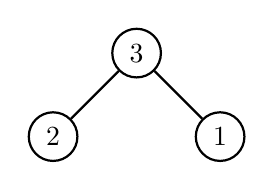
\begin{tikzpicture}[node distance={15mm}, thick, main/.style = {draw, circle}] 
        \node[main] (1) {3}; 
        \node[main] (2) [below left of=1] {2}; 
        \node[main] (3) [below right of=1] {1}; 
        \draw[-] (2) -- (1); 
        \draw[-] (3) -- (1); 
    \end{tikzpicture}
\end{center}

While BUILD-MAX-HEAP' will produce:

\begin{center}
    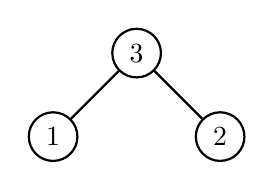
\begin{tikzpicture}[node distance={15mm}, thick, main/.style = {draw, circle}] 
        \node[main] (1) {3}; 
        \node[main] (2) [below left of=1] {1}; 
        \node[main] (3) [below right of=1] {2}; 
        \draw[-] (2) -- (1); 
        \draw[-] (3) -- (1); 
    \end{tikzpicture} 
\end{center}

From CLRS 6.1 \cite{CLRS} we know that the insertion operation is $O(log(n))$. Since we are doing it $n$ times, we get a bound on the runtime of $O(nlog(n))$.

\hfill

\textbf{Problem 7.} Solving the array of integers problem: Radix sort takes an array of $n$ integers, in base $b$, where each number as at most $d$ digits and $d = \lfloor log_b(k) + 1 \rfloor$ where $k$ is the largest number in the array. From \cite{website:3} we know that, when $b$ and $n$ are of the same size magnitude, radix sort will run in $O(d(n+b)) = O(n)$ time. 

First, we go through the array, putting each number in $n$ buckets by number of digits (e.g. [1, 2, 3], [12, 23, 34]...). This takes $O(n)$ steps. The only thing that remains is to sort the numbers within the $n$ buckets. If we assume there are $k_i$ numbers with $i$ digits, then radix will sort these numbers digit by digit in $O(ik_i)$ with $i$ iterations of counting sort over $k_i$ numbers. To sort all the buckets then, we would sum this for $O(\sum ik_i)$. Since we know from the problem that the total number of digits is $n$, we know that $\sum ik_i = n$. Therefore, the total number of steps for the whole algorithm would be $O(n) + O(\sum ik_i) = O(n) + O(n) = O(n)$

\hfill

\textbf{Problem 8.} 


\newpage
\bibliography{citation} 
\bibliographystyle{ieeetr}

\end{document} 
